\section[Data and Preprocessing]{Data, Verification and Shared Preprocessing}
\label{sec:data_def}

\subsection{Official Tiles and Self-Collected Layers}

\textbf{Official data (Attachment~1).} Attachment~1 holds 1000 co-registered triplets, IDs 1001--2000: one pre-flood Sentinel-2 tile with four uint8 bands (B, G, R, NIR), one post-flood GF-3 HH SAR tile with a single uint8 band, and a binary label, each $256\times256$ pixels and stored as GeoTIFF in WGS-84 geographic coordinates at $8.333\times10^{-5}$\,degree per pixel. GeoTIFF tags place the tiles between 112.69 and 116.91$^\circ$E and 28.43 and 29.30$^\circ$N, in four spatial clusters of 512, 450, 22 and 16 tiles -- consistent with the Dongting and Poyang lake basins. The attachment states no event date, and we do not assign one. Class imbalance is strong: pixel-weighted, 18.99\% of the labeled pixels are flooded, yet the median tile carries only 3.76\% flood and 15 tiles carry none, which leaves many tiles with almost no target. The README quotes a mean flood share of 24.5\%; a full traversal of the 1000 label files gives 18.99\%, and the verified value is the one used here.

\textbf{Self-collected data (Hengzhou).} Problems~3--5 use only public layers, listed in Table~\ref{tab:hz_data}. They are reprojected to the 10\,m UTM~49N grid of the Sentinel-1 product (nearest neighbor for classes, bilinear for continuous values) and clipped to the GADM~4.1 boundary, whose geodesic area is 3440.09\,km$^2$.

\textbf{Where the layers come from.} The official triplets are the competition attachment (Attachment~1), not an external download. The Hengzhou layers were downloaded from public archives: Sentinel-1 RTC from Microsoft Planetary Computer; Sentinel-2 L2A and the DEM from Copernicus; land cover from ESA WorldCover; OSM extracts from Geofabrik; population from WorldPop; and the boundary from GADM~4.1. Table~\ref{tab:hz_data} gives the date, resolution and use of each layer.

\begin{table}[!ht]
\centering
\caption{Public data used for Hengzhou}
\label{tab:hz_data}
\small
\begin{tabular}{p{0.27\textwidth}p{0.2\textwidth}p{0.15\textwidth}p{0.265\textwidth}}
\toprule
Layer & Date & Resolution & Use \\
\midrule
Sentinel-1 RTC VV/VH (Planetary Computer)\cite{planetary2026} & 27 Jun, 4 Jul, 16 Jul 2026 & 10\,m grid & $W_0$, flood-time water, model input \\
Sentinel-2 L2A (Copernicus)\cite{copernicuss2_2026} & 31 May 2026 & 10\,m & tested, rejected (Sec.~\ref{sec:q3_verify}) \\
ESA WorldCover v200\cite{worldcover2026} & 2021 & 10\,m & $W_0$, land-cover strata, exposure \\
Copernicus DEM GLO-30\cite{copernicusdem_2026} & -- & 30\,m & relative elevation guard \\
OSM roads, water, places (Geofabrik)\cite{geofabrik2026} & 2026 extract & vector & $W_0$, units, road graph \\
WorldPop constrained\cite{worldpop2026} & 2020 & 100\,m & flooded population \\
GADM 4.1 boundary\cite{gadm2026} & -- & vector & study area \\
\bottomrule
\end{tabular}
\end{table}

Fig.~\ref{fig:data_samples} shows only representative samples, not the full inventory. Panels (a)--(c) are one official triplet: pre-flood optical, post-flood SAR and binary label. Panels (d)--(f) are three Hengzhou layers used downstream: Sentinel-1 VV on 16 July, WorldCover, and WorldPop with OSM roads. The Hengzhou panels use a 150\,m display grid. All analyses use their native grids.

\begin{figure}[!ht]
  \centering
  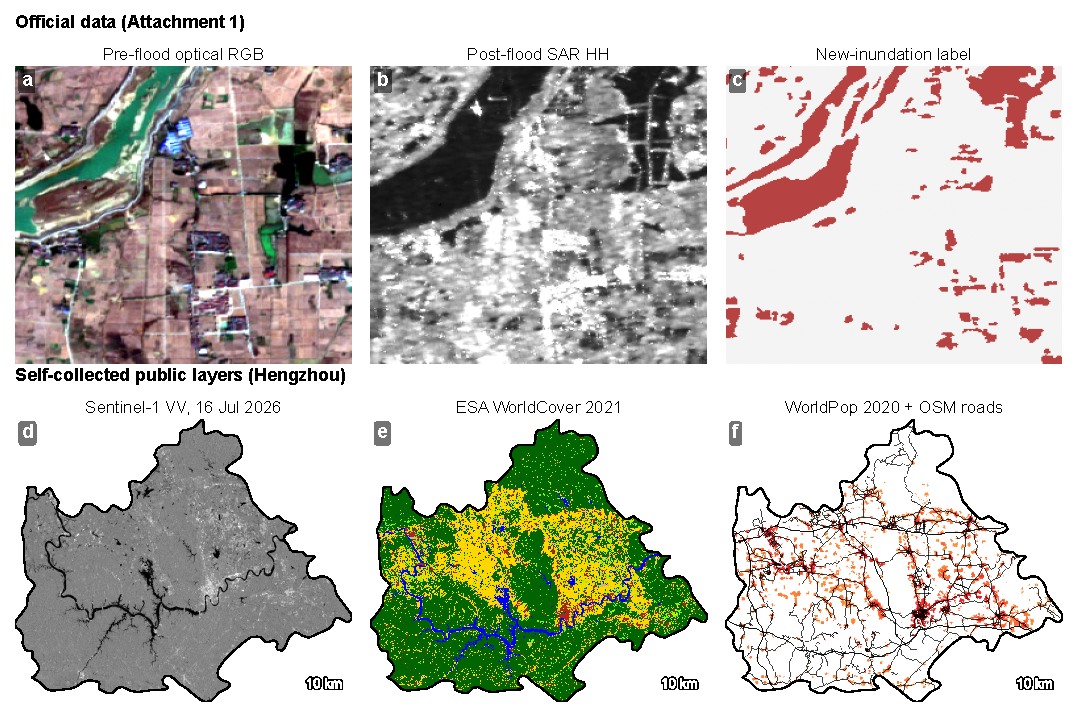
\includegraphics[width=0.90\textwidth,keepaspectratio]{../figures/fig_data_samples.pdf}
  \caption{Representative data samples}
  \label{fig:data_samples}
\end{figure}

Two of its rows needed repair, and the repair belongs to the method. Relative to their geotransform the Sentinel-1 rasters are shifted north--south by 5.4--6.2\,km, and the Sentinel-2 scene cannot be aligned by any translation; both findings, and how they were handled, are reported in Section~\ref{sec:q3_verify}, since they affect only Problems~3--5. Official tiles passed the same test: on the 491 tiles carrying 3--60\% optical water, the shift that best aligns SAR-dark pixels with optical water has a median of $(0,0)$ pixels, and 63.3\% of the tiles align within 2 pixels, which keeps the official triplets on their native grid.

\subsection{What the Official Labels Actually Mark}

The labels are binary and could mean either ``water after the flood'' ($W_1$) or ``new inundation'' ($F$). The difference decides whether a model trained on them learns the quantity the problem asks for. A label that marks $W_1$ must contain the permanent rivers and lakes. A label that marks $F$ must leave them at 0 even though they are dark in the post-flood SAR. We tested this on all 65,491,966 valid pixels with three definitions of pre-flood water ($\mathrm{NDWI}>0$; $\mathrm{NDWI}>0.1$; $\mathrm{NDWI}>0$ and $\mathrm{NDVI}<0$), using the water index of McFeeters~\cite{mcfeeters1996ndwi}.

\begin{figure}[!ht]
  \centering
  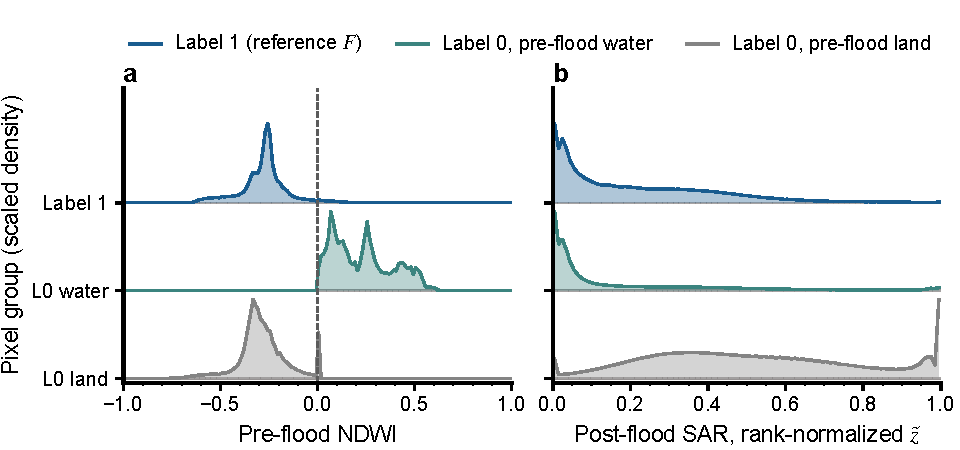
\includegraphics[width=0.90\textwidth,keepaspectratio]{../figures/fig_q1_label_semantics.pdf}
  \caption{Label-semantics test on all valid pixels}
  \label{fig:q1_label_semantics}
\end{figure}

The distributions in Fig.~\ref{fig:q1_label_semantics} separate cleanly. Panel (a) shows pre-flood NDWI for three pixel groups: label-1 pixels sit almost entirely below zero, and only 2.37\% of them had $\mathrm{NDWI}>0$ before the event (2.06\% under the strict definition). Panel (b) shows post-flood SAR brightness: pre-flood water pixels that carry label 0 are just as dark as the flooded pixels, and 70.1\% of them fall below the dark threshold $\tilde z<0.2$. Pre-flood water is therefore still water after the flood, but the labels exclude it. The labels mark newly inundated area with permanent water set to 0, and this holds for all three definitions. Problems~1--2 therefore learn $F$ directly, and Problem~3, where no labels exist, builds $W_0$ independently and subtracts it.

\subsection{Area Definitions and Their Set Logic}

The four sets of \eqref{eq:def_F} are related by $W_1=F\cup(W_0\cap W_1)$ and $W_0=(W_0\cap W_1)\cup R$ with $R=W_0\setminus W_1$, which gives
\begin{equation}
A_{net}=|W_1|_a-|W_0|_a=A_{new}-|R|_a\le A_{new},
\label{eq:net_identity}
\end{equation}
where $|\cdot|_a$ is the area-weighted size of a set. Comparing an estimate $\hat F$ with the reference $F$ splits the area error into false alarms and misses,
\begin{equation}
\hat A-A=|\hat F\setminus F|_a-|F\setminus\hat F|_a=|\mathrm{FP}|_a-|\mathrm{FN}|_a .
\label{eq:fpfn_identity}
\end{equation}
Fig.~\ref{fig:q1_set_logic} draws both identities.

\begin{figure}[!ht]
  \centering
  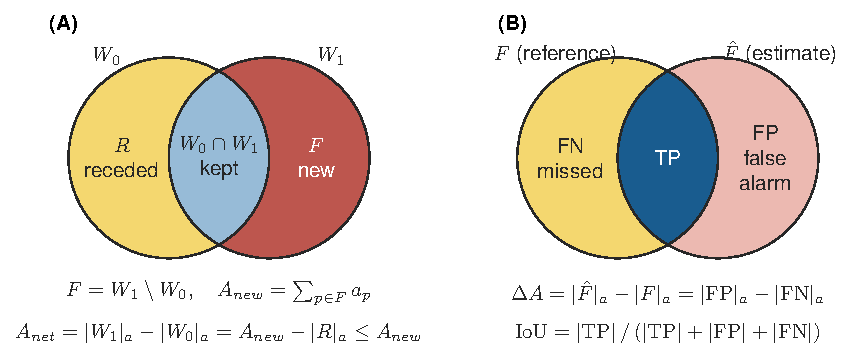
\includegraphics[width=0.90\textwidth,keepaspectratio]{../figures/tikz_q1_set_logic.pdf}
  \caption{Set logic of the area definitions}
  \label{fig:q1_set_logic}
\end{figure}

Panel (a) of Fig.~\ref{fig:q1_set_logic} explains why the net increase can be negative while new inundation is positive: any receded water $R$ (drained ponds, a lower river stage) is subtracted from $A_{new}$, and this happens in Hengzhou. Panel (b) explains why IoU alone is not enough for this problem. Identity \eqref{eq:fpfn_identity} lets a model with many false alarms and as many misses report an almost exact total area. Area error is always reported together with IoU here, split by land cover into FP and FN parts.

\subsection{Shared Preprocessing}

\textbf{Pixel area.} The ground area of a geographic pixel with center latitude $\varphi_p$ and angular sizes $\Delta\lambda,\Delta\varphi$ follows from the WGS-84 meridian and prime-vertical radii, with $a=6378137$\,m and $e^2=0.00669438$:
\begin{equation}
\begin{split}
M(\varphi)&=\frac{a(1-e^2)}{(1-e^2\sin^2\varphi)^{3/2}},\qquad
N(\varphi)=\frac{a}{(1-e^2\sin^2\varphi)^{1/2}},\\
a_p&=M(\varphi_p)\,\Delta\varphi\cdot N(\varphi_p)\cos\varphi_p\,\Delta\lambda .
\end{split}
\label{eq:pixel_area}
\end{equation}
On the official tiles $a_p$ ranges from 74.78 to 75.41\,m$^2$ and the mean tile area is 4.913\,km$^2$. On the Hengzhou UTM grid $a_p=100/k_p^2$\,m$^2$ with the UTM point scale factor $k_p$. Every area in this paper is $\sum a_p$ over a mask.

\textbf{Geometry.} Label, SAR and optical tie points differ by at most 0.47 pixel. Nine label tiles have an anisotropic pixel size ($7.9119\times10^{-5}$ by $8.3349\times10^{-5}$ degree) and are resampled by nearest neighbor onto the SAR grid. Pixels outside the label footprint are excluded from all metrics.

\textbf{SAR normalization and speckle.} The radiometric scale of the GF-3 values is unknown (Assumption~2), and each tile is rank-normalized with its own 2\% and 98\% quantiles,
\begin{equation}
z_p=\mathrm{clip}\!\left(\frac{I_p-Q_2}{Q_{98}-Q_2+\epsilon},0,1\right),\qquad \epsilon=10^{-6},
\label{eq:rank_norm}
\end{equation}
and then filtered by the Lee filter~\cite{lee1980local} on a $5\times5$ window $\Omega_p$:
\begin{equation}
\begin{split}
\tilde z_p&=\bar z_p+k_p\,(z_p-\bar z_p),\qquad
k_p=\max\!\left(0,\ 1-\frac{C_u^2}{C_{z,p}^2}\right),\\
C_{z,p}^2&=\frac{\mathrm{Var}_{\Omega_p}(z)}{\bar z_p^2+\epsilon},\qquad
C_u=\frac{1}{\sqrt L}.
\end{split}
\label{eq:lee}
\end{equation}
The equivalent number of looks $L$ is estimated per tile as the median of $\bar z^2/\mathrm{Var}(z)$ over the 10\% most homogeneous $7\times7$ windows; its median over the official tiles is 31.0. The filter smooths homogeneous areas ($k_p\to0$) and keeps edges ($k_p\to1$), which matters for narrow flooded channels. Because \eqref{eq:rank_norm} uses only the tile itself, no information crosses the validation folds.

\textbf{Optical indices and features.} The validity mask is $m_p=\mathbb 1[\max(B,G,R,N)>0]$; 60 official tiles have more than 5\% invalid optical pixels. From the bands we compute $\mathrm{NDWI}=(G-N)/(G+N+\epsilon)$, $\mathrm{NDVI}=(N-R)/(N+R+\epsilon)$ and the brightness $(B+G+R+N)/1020$. The pixel classifier of Problem~1 uses 19 features: $z$, $\tilde z$, local mean and standard deviation of $\tilde z$ on $3\times3$, $7\times7$ and $15\times15$ windows, the $7\times7$ minimum of $\tilde z$, the three indices and the $7\times7$ mean NDWI, the four scaled bands, $m_p$, and the interaction $\tilde z(1-\mathrm{NDWI}^+)$, which encodes ``dark now and not water before''\cite{deepseek2026,qwen2026,doubao2026}.
